\chapter{Estado del arte}
\label{chap:estadoarte}

\lettrine{E}{n este capítulo} se realiza un análisis de las aplicaciones y herramientas existentes que pueden aportar soluciones para abordar la problemática comentada en este proyecto.

El objetivo no es ofrecer una revisión exhaustiva, sino actualizar el estado de las alternativas ya tratadas en el trabajo previo \cite{TFGAdrianGarcia2025} y añadir otras herramientas que, por su evolución reciente o por su encaje funcional, resultan relevantes para valorar la propuesta de este proyecto.

\section{Aplicaciones analizadas}
\label{sec:arte-tfg}

Las aplicaciones se agrupan por funcionalidad para facilitar la comparación. Se ha revisado que las aplicaciones que ya han sido comentadas en el trabajo previo \cite{TFGAdrianGarcia2025} no han sufrido cambios significativos en su enfoque o funcionalidades, por lo que se mantienen las conclusiones previas sobre su encaje funcional. Como el alcance de la solución se ha ampliado, se han investigado nuevas herramientas que puedan aportar funcionalidades complementarias o enfoques alternativos para la gestión de emergencias, la representación geoespacial y la participación ciudadana, especialmente en lo relativo a la aplicación móvil para la ciudadanía, que es un aspecto reforzado en esta nueva etapa del proyecto.

\subsection{Gestión de incidencias y coordinación}

\subsubsection{Jira}

Jira \cite{jira} es una plataforma de gestión de incidencias y proyectos útil para crear, priorizar y asignar tickets. Sin embargo, no aporta representación geoespacial nativa, por lo que su encaje en emergencias es parcial.

\subsubsection{Asana}

Asana \cite{asana} ofrece gestión de tareas, prioridades y colaboración en equipo. Su principal carencia para este caso es que no integra mapas ni soporte geográfico.

\subsubsection{Microsoft Teams}

Microsoft Teams \cite{microsoft_teams} ayuda a organizar equipos y comunicación, pero no ofrece geolocalización ni procesos específicos para emergencias.

\subsubsection{Odoo}

Odoo \cite{odoo} es flexible y modular, pero requiere personalización para ajustarse a flujos de coordinación de emergencias y a soporte geográfico.

\subsection{Cartografía y monitorización}

\subsubsection{Global Forest Watch - Fires}

Global Forest Watch Fires \cite{gfw_fires} aporta cartografía y alertas sobre incendios a partir de datos satelitales, pero no está pensada para coordinar recursos humanos ni para participación ciudadana.

\subsubsection{InciWeb}

InciWeb \cite{inciweb} centraliza información sobre incidentes y grandes incendios con mapas e informes, pero no incorpora avisos colaborativos ni gestión táctica de equipos.

\subsubsection{Google Maps}

Google Maps \cite{google_maps} permite mostrar alertas geoespaciales y ofrece una cartografía muy amplia, aunque no resuelve por sí mismo la gestión de despliegue ni el flujo de incidentes.

\subsubsection{PCAM Gestión}

PCAM Gestión \cite{pcam_gestion} ofrece avisos, asignación de personal y notificaciones en el ámbito de la protección civil, aunque con capacidades geoespaciales limitadas.

\subsubsection{XeoCode Lite}

XeoCode Lite \cite{xeocode_lite} es una herramienta interna y privada de la Xunta de Galicia. Permite consultar el origen y evolución de incendios, recursos asignados y cartografía asociada, pero no expone información funcional al público ni permite participación ciudadana directa.

\subsection{Participación ciudadana y avisos públicos}

\subsubsection{Línea Verde}

\begin{figure}[H]
  \centering
  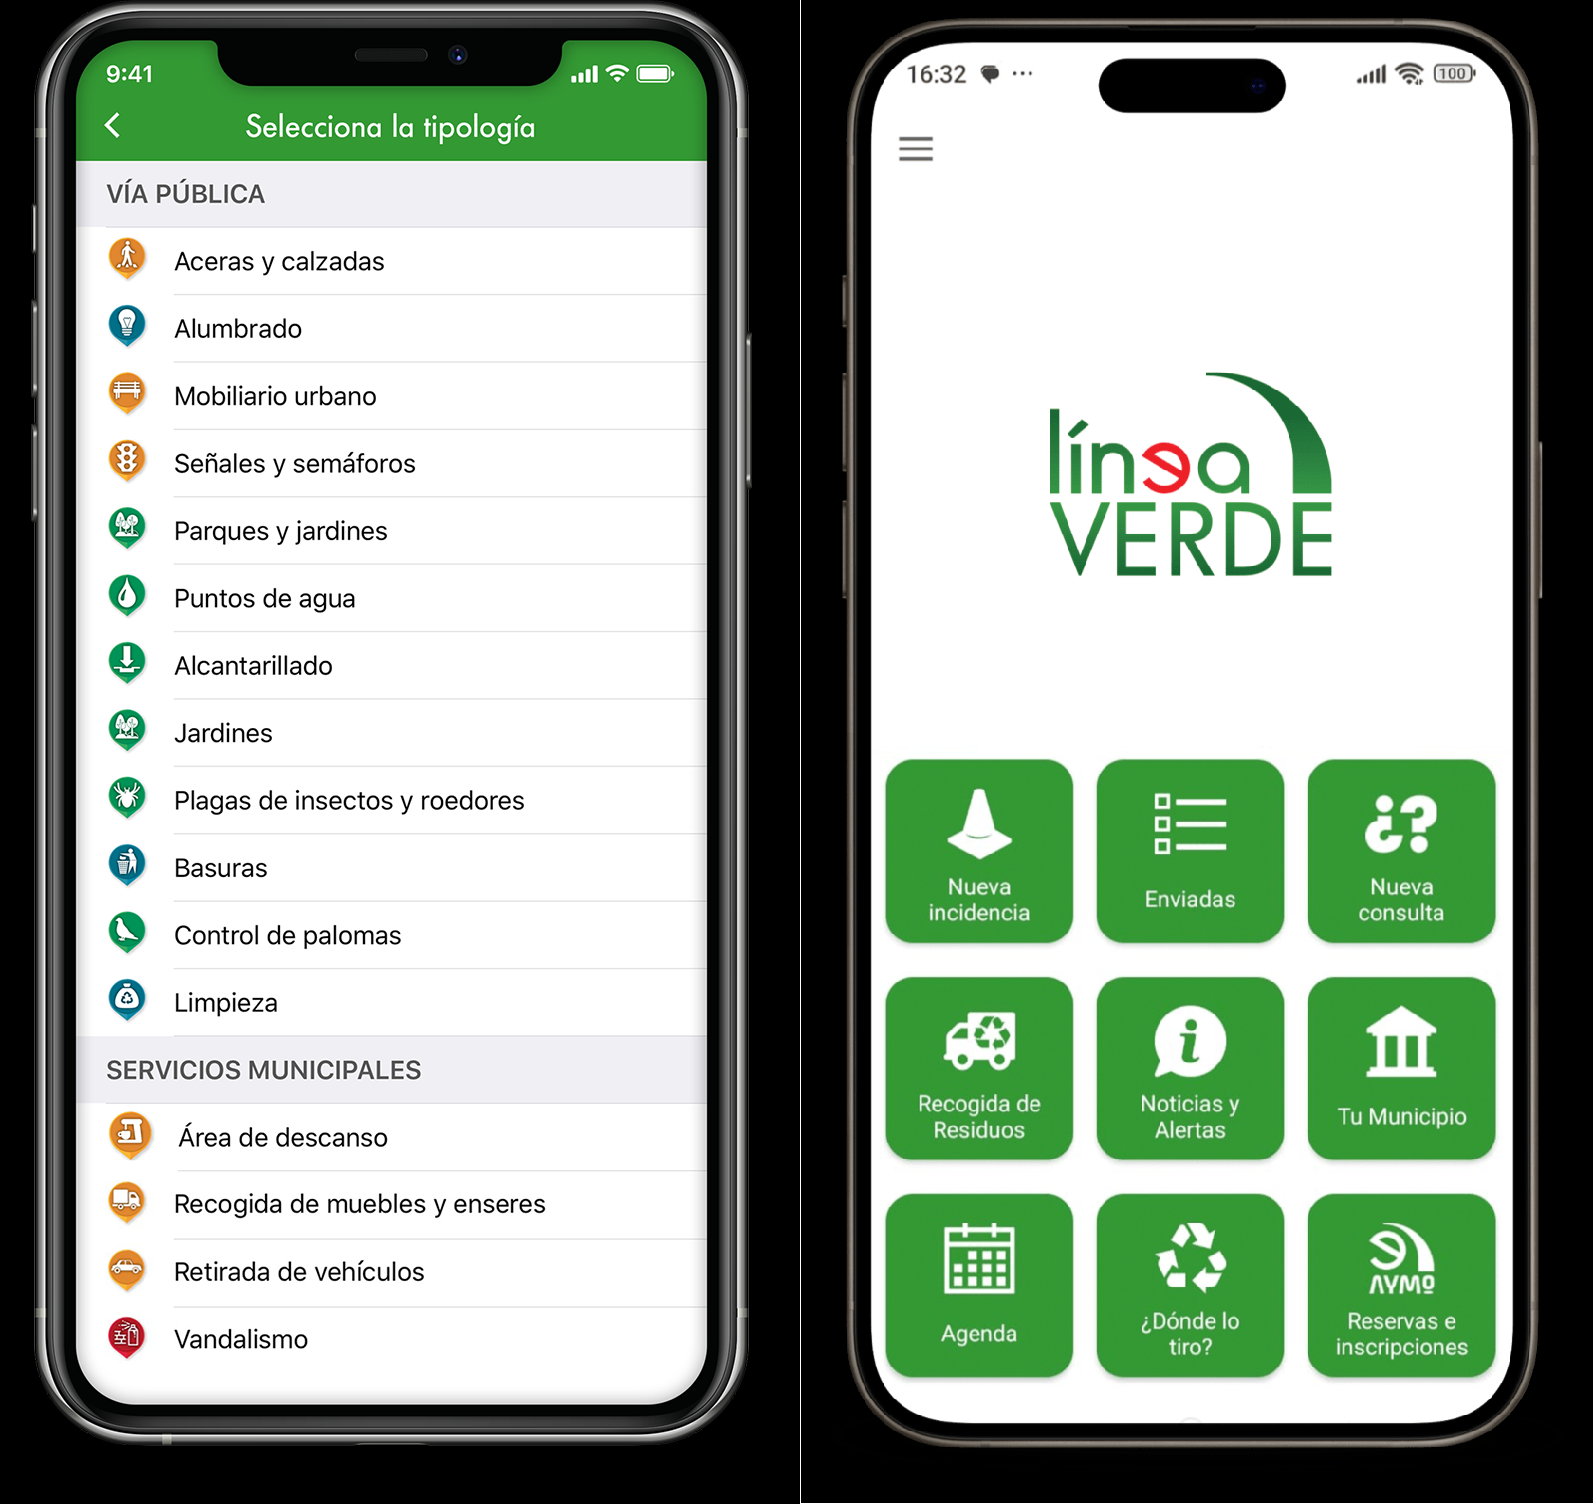
\includegraphics[width=0.7\textwidth]{imaxes/arte/linea_verde.png}
  \caption{Vista de la app Línea Verde}
  \label{fig:LíneaVerde}
\end{figure}

Línea Verde \cite{linea_verde} es una plataforma municipal de participación ciudadana y gestión de incidencias. Está bien orientada a comunicación con la administración, pero su foco es urbano y no operativo para emergencias.

\subsubsection{S.O.S Emergencias}

\begin{figure}[H]
  \centering
  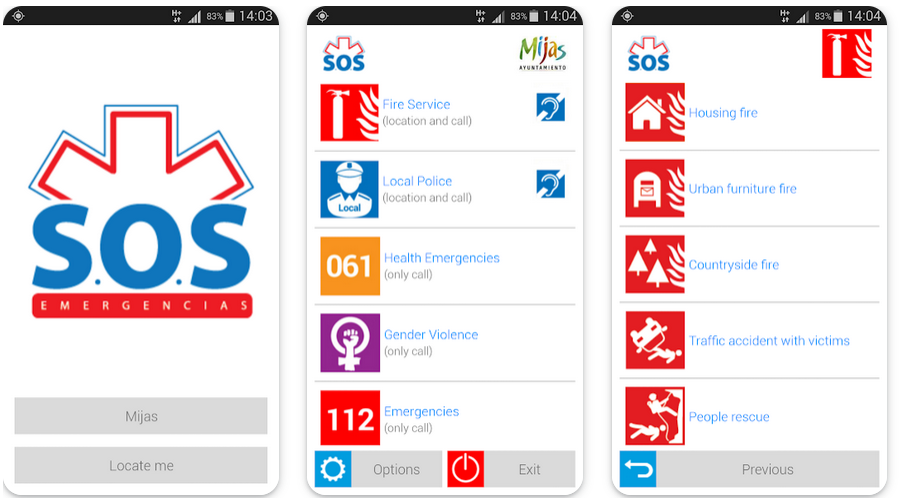
\includegraphics[width=0.7\textwidth]{imaxes/arte/sos_emergencias.png}
  \caption{Vista de la app S.O.S Emergencias}
  \label{fig:SOSEmergencias}
\end{figure}

S.O.S Emergencias \cite{sos_emergencias} es una aplicación móvil orientada a la notificación y gestión básica de emergencias. Aporta una aproximación más directa al ámbito de alertas, aunque no integra una visión completa de coordinación geoespacial y despliegue de recursos.

\section{Iniciativas públicas recientes}
\label{sec:arte-public}
En un comunicado, la Xunta de Galicia ha anunciado la ampliación de mecanismos de detección temprana de incendios forestales mediante la creación de una nueva app para la ciudadanía junto con el uso de cámaras de videovigilancia \cite{xunta_deteccion_incendios_2026}.

Esta aplicación combina un canal para notificaciones tempranas, sensores y cámaras para observación remota y procesamiento automatizado con IA para priorizar alertas y detectar anomalías. Todo ello ayuda a la notificación y coordinación de emergencias en tiempo real.

Funcionalmente esta nueva app parece converger mucho con el dominio funcional de la solución precedente \cite{TFGAdrianGarcia2025}: reportes ciudadanos, integración de sistemas de información dispares como avisos ciudadanos y meteorológicos y también cuenta con representación geoespacial; a efectos prácticos la solución de la Xunta incorpora muchas de las ideas que se prototiparon en el trabajo previo.

Algunas diferencias clave respecto a la solución inicial son que la aplicación añade una capa de hardware y vigilancia (cámaras/sensores) y está diseñada para integrarse en procedimientos administrativos y operativos a escala autonómica. Por otro lado, aquella primera propuesta aporta un énfasis en la coordinación táctica, como la asignación de recursos, la gestión por cuadrantes y el soporte a decisiones de despliegue en campo.

Como comentario crítico, cabe destacar la coincidencia temática que resalta la relevancia del problema abordado en la propuesta previa y demuestra que las soluciones planteadas tienen aplicación real. Ambas aproximaciones son complementarias y evidencian la necesidad de soluciones integrales que aborden todo el ciclo de gestión de emergencias, desde la detección hasta la coordinación en campo.

\section{Conclusión}
Las aplicaciones analizadas ofrecen soluciones parciales en las tres dimensiones de interés: gestión de avisos, representación geoespacial y coordinación de equipos. Ninguna de las herramientas revisadas integra de forma nativa las tres capacidades con enfoque ciudadano-operativo y despliegue de recursos; esto evidencia el hueco funcional que aborda la propuesta de este trabajo.

La tabla comparativa 3.1 resume las funcionalidades analizadas para resaltar fortalezas y carencias de cada alternativa:

\begin{table}[H]
  \centering
  \resizebox{\textwidth}{!}{
    \rowcolors{2}{white}{udcgray!25}
    \begin{tabular}{c|c|c|c|c|c|c|c|c}
      \rowcolor{udcpink!25}
      &
      \begin{tabular}[c]{@{}l@{}}Visualización \\ geográfica\end{tabular} &
      \begin{tabular}[c]{@{}l@{}}Datos \\ meteorológicos\end{tabular} &
      \begin{tabular}[c]{@{}l@{}}Gestión de \\ personal y recursos\end{tabular} &
      \begin{tabular}[c]{@{}l@{}}Plan gratuito \\ suficiente\end{tabular} &
      \begin{tabular}[c]{@{}l@{}}Plugins \\o margen de mejora\end{tabular} & 
      \begin{tabular}[c]{@{}l@{}}Sistema de avisos \\o notificaciones\end{tabular} &
      \begin{tabular}[c]{@{}l@{}}Multi-\\emergencia\end{tabular} &
      \begin{tabular}[c]{@{}l@{}}App \\ móvil\end{tabular} \\
      \textit{Jira} &  &  & \checkmark & \checkmark & \checkmark & \checkmark & \checkmark & \checkmark \\
      \textit{Asana} &  &  & \checkmark & \checkmark & \checkmark & \checkmark & \checkmark & \checkmark \\
      \textit{Línea Verde} & \checkmark &  & \checkmark & \checkmark & & \checkmark & \checkmark & \checkmark \\
      \textit{SOS Emergencias} & & & \checkmark & \checkmark & & \checkmark & \checkmark & \checkmark \\
      \textit{Global Forest Watch - Fires} & \checkmark & \checkmark &  & \checkmark &  & \checkmark &  &  \\
      \textit{InciWeb} & \checkmark &  &  & \checkmark &  &  &  &  \\
      \textit{Google Maps} & \checkmark &  &  & \checkmark & \checkmark &  &  & \checkmark \\
      \textit{Microsoft Teams} &  &  & \checkmark & \checkmark & \checkmark & \checkmark & \checkmark & \checkmark \\
      \textit{Odoo} &  &  & \checkmark & \checkmark & \checkmark & \checkmark & \checkmark & \checkmark \\
      \textit{PCAM Gestión} & \checkmark &  & \checkmark &  & \checkmark & \checkmark & \checkmark & \checkmark \\
      \textit{XeoCode Lite} & \checkmark & ? & \checkmark & ? & ? & ? & ? & ? \\
      \textit{Xunta (nueva app)} & \checkmark & \checkmark &  & \checkmark &  & \checkmark &  & \checkmark \\
    \end{tabular}}    
    \caption{Tabla comparativa entre aplicaciones}
    \label{tab:comparativa}
\end{table}
